\documentclass{article}

\usepackage[utf8]{inputenc}
\usepackage{geometry}
\usepackage{algorithm}
\usepackage{algpseudocode}
\usepackage{graphicx}

\title{Algoritmo: Buscar el par de puntos mas cercano en espacio n-dimensional}
\author{Sergio García Prado}


\begin{document}

\begin{titlepage}
	\centering
	{\scshape\LARGE Universidad de Valladolid \par}
	\vspace{1cm}
	{\scshape\Large Algoritmo Divide y vencerás\par}
	\vspace{1.5cm}
	{\huge\bfseries Par de puntos más cercano en espacio n-dimensional\par}
	\vspace{2cm}
	{\Large\itshape Sergio García Prado\par}


% Bottom of the page
	{\large \today\par}
\end{titlepage}

\section{Introducción}

	\paragraph{}
	El problema que se va a analizar se basa en encontrar los dos puntos más cercanos entre un conjunto de puntos pertenecientes en un espacio n-dimensional. Es una condición obligatoria que todos los puntos pertenezca a la misma dimensión ya que de no ser así no tendría sentido comparar sus distancias.

	\paragraph{}
	Existen distintos enfoques para resolver este problema. El mas simple pero a la vez menos eficiente de todos se basa en comparar todos los puntos con todos e ir guardando los dos que menor distancia tienen entre sí. Esta solución tiene un coste de O(n2) algo que podemos mejorar si nos damos cuenta de algunos detalles mediante algoritmos del tipo divide y vencerás.

	\paragraph{Motivos por los que usar divide y vencerás}

		\begin{enumerate}

			\item
			Los puntos mas cercanos en el espacio por la propia definición de cercanía van a estar en una región próxima del espacio. Este es el motivo por el cual nos podemos ahorrar comparar dos puntos que están muy alejados en el mapa.
			\item
			Si encontramos un mínimo en un subconjunto del espacio y este lo es también para todos los subconjuntos que contienen a este, entonces habremos encontrado el mínimo de todo el espacio.

		\end{enumerate}

\section{Solución}

	\paragraph{}
	La solución que se ha escogido es la de realizar particiones binarias en el espacio recursivamente hasta tener subconjuntos de pequeño tamaño (En la implementación propuesta como ejemplo se ha fijado en conjuntos de 10 puntos.) para después compararlos utilizando un algoritmo boraz que nos asegura el mínimo local de cada subconjunto. Lo siguiente es quedarse con el mínimo de las dos particiones binarias y analizar los puntos que se quedaron en la frontera de las dos particiones ya que puede darse el caso de que el par de puntos con distancia mínima contuviese el punto 1 en la particion 1 y el punto 2 en la partición 2. De no ser por la parte de combinación estos casos no se estudiarían y podría darse el caso de que el mínimo encontrado no fuera el real.

	\paragraph{}
	Las explicaciones se van a exponer en un espacio de 3 dimensiones pero estas son extrapolables cualquier número de dimensiones.

	\subsection{Divide}
		\paragraph{}
		Lo que intentamos conseguir al dividir el espacio en particiones binarias recursivamente es agrupar los puntos que están más próximos para así intentar prescindir del mayor número de comparaciones innecesarias. Para ello se pueden tomar distintos enfoques:
		
		\begin{itemize}
		
			\item 
			El primero de ellos consiste en hacer la partición siempre en la misma dimensión. Este enfoque tiene la ventaja de que tan solo hay que ordenar los elementos una vez, ya que al no tener que cambiar de dimensión la ordenación se mantiene. Pero aún así esto es menos eficiente ya que no se consigue la meta deseada que era agrupar los puntos cercanos en conjuntos. En este caso al solo depender de una de las dimensiones en las otras pueden tener valores muy diferentes por lo que al producirse la fusión se tienen que evaluar muchos más puntos. Esto se ilustra en la figura \ref{same_dim}. 
			
			\item 
			La segunda solución consiste en que en cada nivel de recursión se cambie la dimensión en la que se particionan los puntos, lo que conlleva a una reordenación de los mismos respecto a dicha dimensión. La carga de trabajo en este caso es mayor pero la división que se consigue es mucho más homogénea en cuanto a distancia lo que nos da una gran ventaja al fusionar los distintos subconjuntos. Esto se ilustra en la figura \ref{different_dim}. 

		\end{itemize}



	\begin{figure}[ht!]
		\centering
		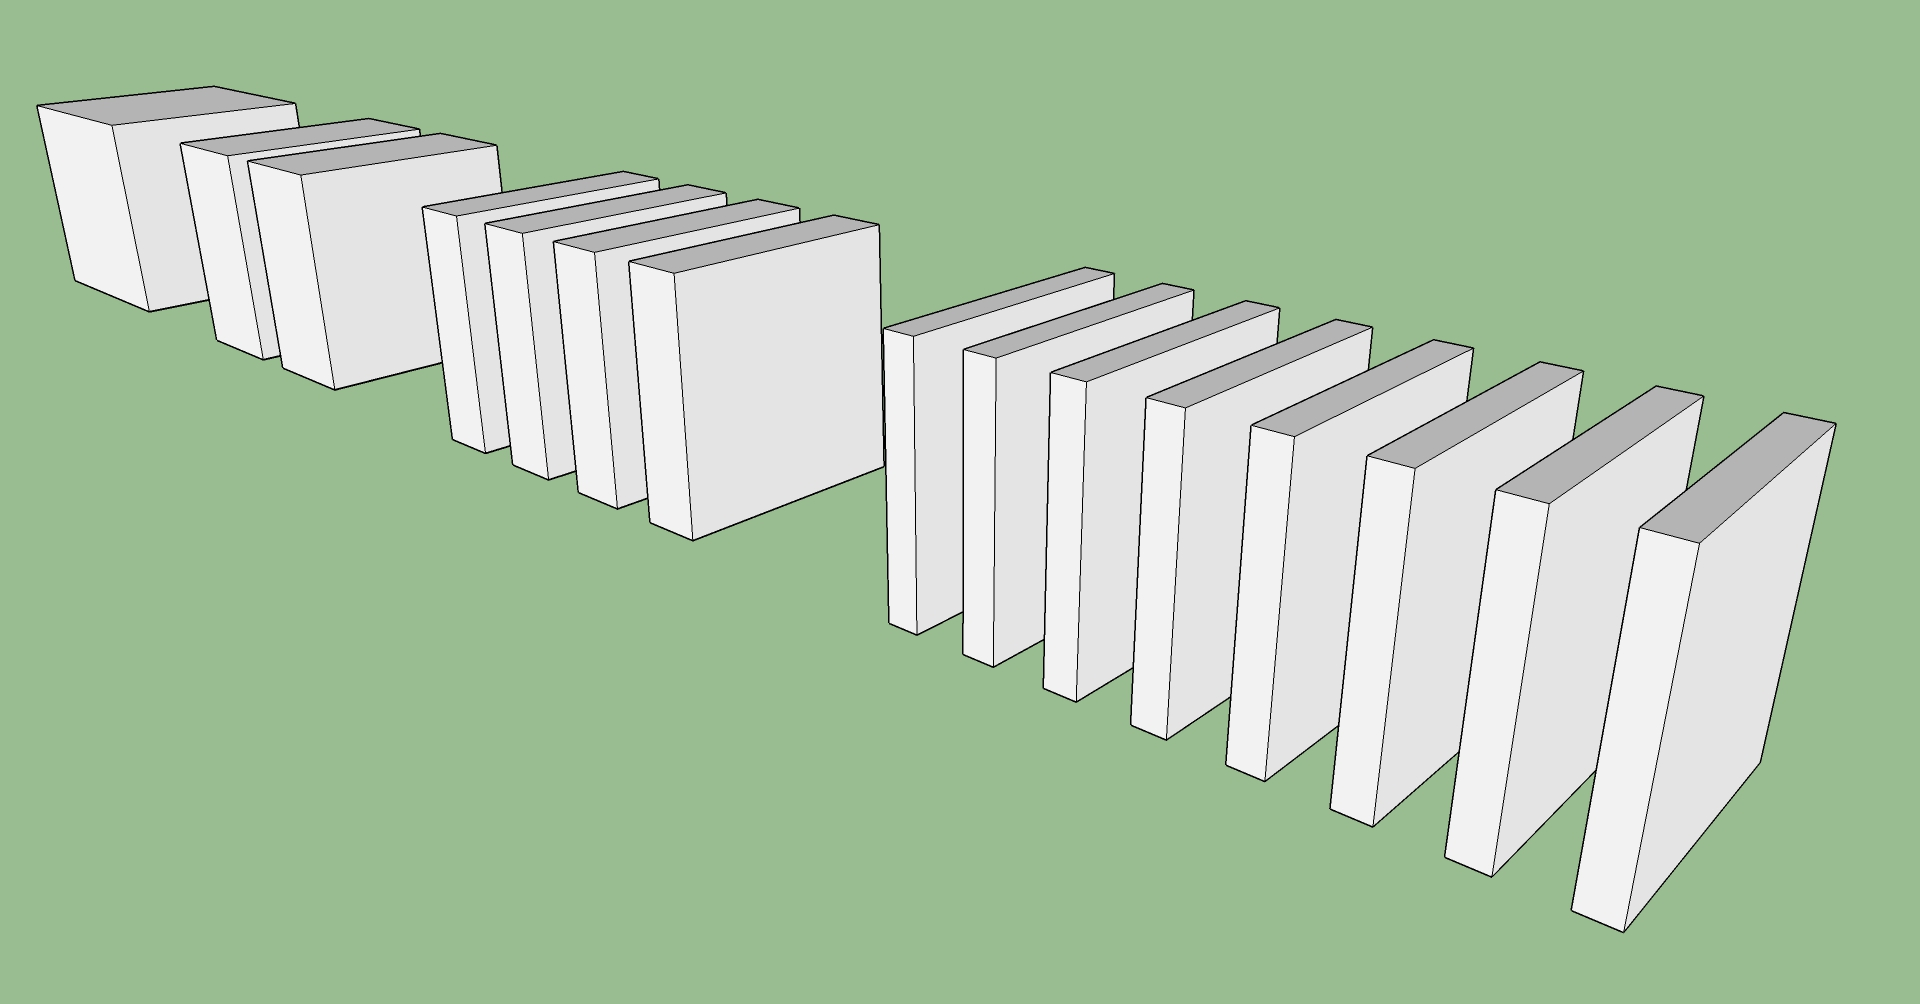
\includegraphics[width=120mm]{cube_division_1.jpg}
		\caption{Particionamiento en la misma dimensión \label{same_dim}}
	\end{figure}

	\begin{figure}[ht!]
		\centering
		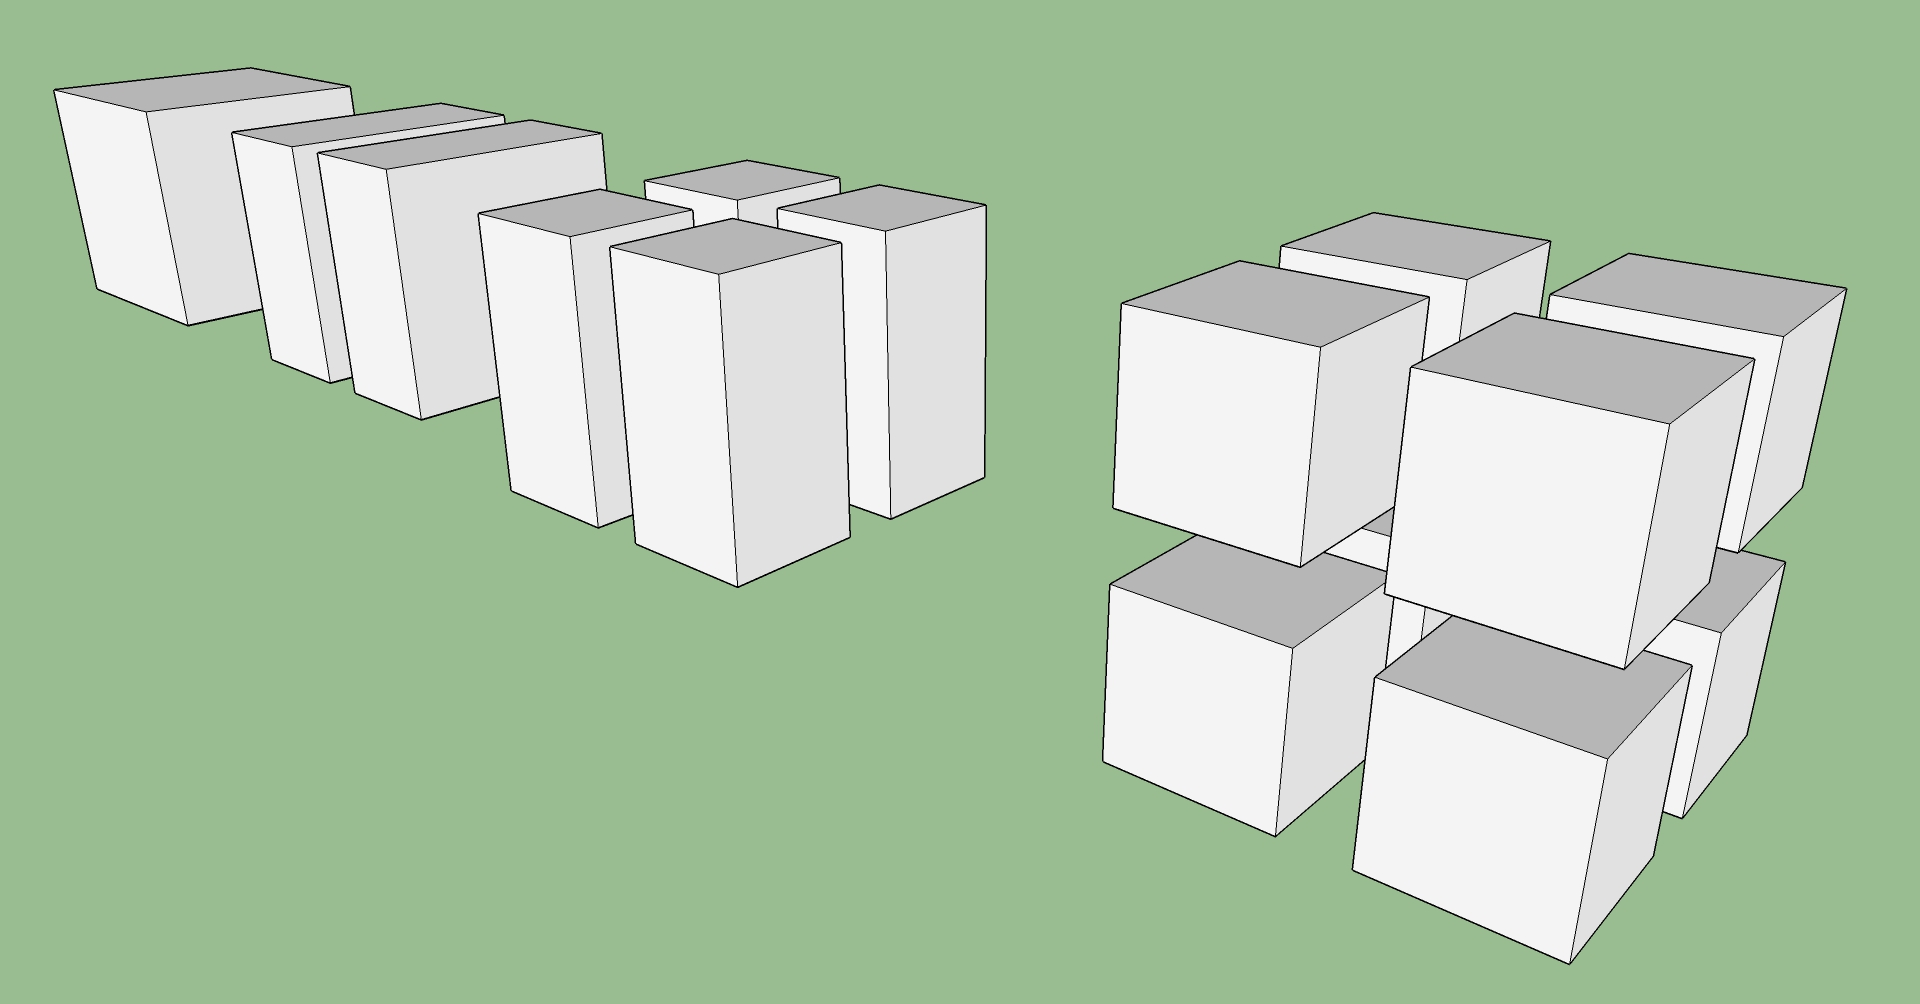
\includegraphics[width=120mm]{cube_division_2.jpg}
		\caption{Particionamiento en distintas dimensiones \label{different_dim}}
	\end{figure}


	\subsection{Venceras}
		\paragraph{}





\section{Pseudocódigo}
% Insert the algorithm
\begin{algorithm}
    \caption{Compute sum of integers in array}
        \label{array-sum}
        \begin{algorithmic}[1]
            \Procedure{ClosestPair}{$A$}
            \State $sum = 0$
            \For {each integer $i$ in $A$}
                \State $sum = sum + i$
            \EndFor
            \State Return $sum$
            \EndProcedure
        \end{algorithmic}
    \end{algorithm}
\section{Análisis de crecimiento}

\end{document}
